\section{Gestion de project}

\subsection{Planning prévionnel}

J'ai tout d'abord élaboré un diagramme de Gantt (voir annexe \ref{appendix:gantt}) pour plannifier les différentes tâches que à faire pour la réalisation du projet, de la conception à la mise en production. Pour planifier les différentes tâches je me suis inspiré de la notion de \textit{sprints} de la méthode Agile Scrum \cite{scrum}. Un sprint, tel qu'utilisé dans la gestion de ce projet, est une phase de developpement de l'application d'une durée de une semaine. Au terme d'un sprint, les fonctionnalités développées durant la semaine doivent être terminées, testées et prête à être disponible en production.

\begin{figure}
  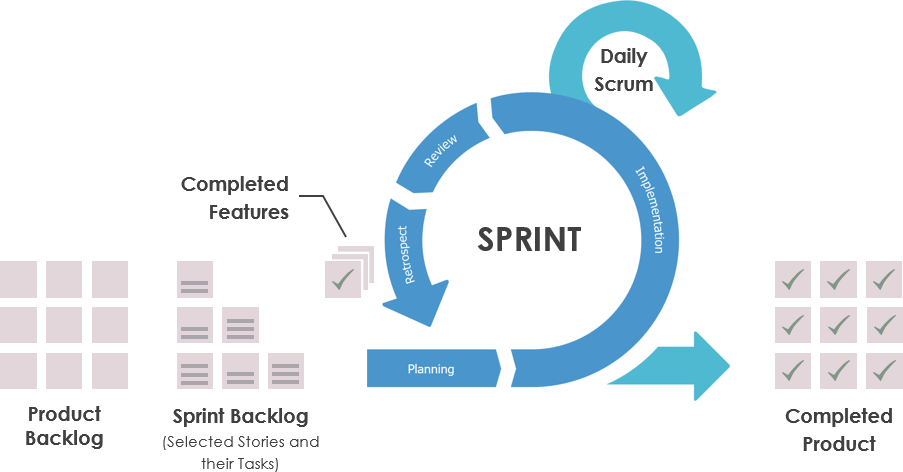
\includegraphics[width=.7\linewidth]{content/imgs/scrum_sprint.png}
  \caption{Sprint Scrum}
\end{figure}

Sur les 12 semaines de stage, 7 semaines ont été consacrées au developement de l'application. J'ai donc, en début de projet, défni les fonctionnalités de  chacun des 7 sprints correspondant aux 7 semaines. Les premières semaines ont été consacrées à la prise en main du sujet, aux recherches, à l'élaboration du cahier des charges et à la conception de l'architecture de l'application. Les deux dernières semaines ont été reservées au déploiement final de l'application sur le \textit{Play Store} et à ce rapport.

Le planning effectivement suivi du projet, après modification de celui-ci au cours du projet, est disponible dans la partie \nameref{chapter:bilan} de ce rapport.

\subsection{Gestion de version (git)}

J'ai choisi d'utiliser le système de gestion de version \textit{Git} avec le service d'hébergement \textit{Github} afin de donner un accès rapide et complet au travail effectué sur l'application à mon enseignant-référent et à ma superviseure de stage.

\textit{Github} m'a aussi permis de créer des points de sauvergarde du projet, appelés \textit{release}, permettant de télécharger le code source des versions majeures de l'application avec le fichier d'installation pour les appareils Android. Les \textit{release} sont aussi accompagnées d'une description de ce qui a changé depuis la dernière version (voir l'annexe \ref{appendix:release}, exemple de la dernière \textit{release} du projet).











% eof
